% importa variabili globali
% definizione variabili globali
\def\GRUPPO {\textit{DazzleWorks}}

\def\PROGETTO {\textbf{Premi}}

\def\COMMITTENTE {Prof. Vardanega Tullio, \\ & Dr. Cardin Riccardo}

\def\EMAIL {dazzleworksgroup@gmail.com}

\def\LOGO {../../template/img/logo.png}

\def\INTESTAZIONE {../../template/img/intestazione.png}
\def\PIEDIPAGINA {../../template/img/piedipagina.png}

\def\G {{\small $_G$}}



% definizione variabili locali
\def\DOCUMENTO{Specifica tecnica}
\def\VERSIONE{1.0.0}

\def\DESCRIZIONE{<Info documento}

\def\REDATTORE {<Redattore>}
\def\VERIFICATORE {<Verificatore>}
\def\RESPONSABILE {Carraro Nicola}

\def\USO {Esterno}

\def\DISTRIBUZIONE {\GRUPPO{}\\ & \COMMITTENTE{}\\}

\def\DESCRIZIONE {Specifica tecnica e architettura dell'applicazione Premi}


% abilita (true) / disabilita (false) indice, lista tabelle, lista figure
\def\INDICE	{true}
\def\TABELLE {true}
\def\FIGURE {true}


% importa struttura
\documentclass[a4paper]{article}

% ----- definizioni -----
\def\TITLE		{\mbox{\GRUPPO}}
\def\SUBTITLE	{\SIGLA, \PROGETTO}


% ----- nuovi comandi -----
% fornisce il caption per riferirsi ad una particolare sezione
\newcommand{\numref}[1]{\textsf{\textsl{``\nameref{#1}'' (\ref{#1})}}}


% ----- package -----
\usepackage[T1]{fontenc}   % codifica dei font in uscita
\usepackage[utf8x]{inputenc}   % lettere accentate da tastiera
\usepackage[italian]{babel}   % lingua principale del documento
\usepackage[a4paper, top= 3cm, bottom= 3cm, left= 3cm, right= 3cm, bindingoffset= 5mm]{geometry} % impostazione margini

\usepackage{amssymb} %

\usepackage{booktabs} % comandi aggiuntivi per le tabelle

\usepackage{calc} % espressioni aritmetiche
\usepackage{caption} % descrizione figure, ecc
\usepackage{chapterbib} % inclusione delle bibliografie

\usepackage{datatool} % manipolazione dati
\usepackage{dcolumn} % array in tabular

\usepackage{epstopdf} % conversione eps--> pdf
\usepackage{enumitem} % personalizzazione liste
\usepackage{eurosym} % simbolo euro

\usepackage{fancyhdr}   %personalizzazione dello stile
\usepackage{float} % definizione di oggetti floating (es. figure, tabelle)
\usepackage[bottom]{footmisc} % personalizzazione note

\usepackage[toc]{glossaries}	% glossario
\usepackage{graphicx, subfigure} % pacchetto grafica testo
\usepackage{grffile} % estende gestione filename graphic

\usepackage[colorlinks=true, urlcolor=blue, citecolor=black, linkcolor=black, hyperindex, breaklinks]{hyperref} % gestione dei link

\usepackage{ifthen}	% costrutto ifthenelse

% \usepackage{listings} % inserimento pezzi di codice
\usepackage{longtable} % tabelle su più pagine

\usepackage{pgf} % grafica postscript e PDF
\usepackage{pgfplots}	% composizione di grafici
\pgfplotsset{/pgf/number format/use comma, compat=newest}	% opzioni per i grafici

\usepackage{multirow} % span multiriga

\usepackage{tabularx, array} % crea paragrafi a colonne
\usepackage{titlesec} % personalizzazione titoli
\usepackage{tikz} % gestione delle formule
\usepackage{totpages} % conta numero pagine

\usepackage{soul} % gestione letterspacing
\usepackage{subfigure} % gestione delle sottofigure

\usepackage{verbatim} % inserimento testo verbatim, non interpretato

\usepackage{wallpaper} % gestione background

\usepackage{xspace} % spazi automatici per le macro


% ----- posizione etichette -----
\captionsetup{tableposition=top, figureposition=bottom, font=small}


% ----- glossario -----
\loadglsentries{../../glossario/glossario.tex}
\renewcommand*{\glssymbolsgroupname}{Simboli}


% ----- stile pagina -----
\pagestyle{fancy}

	% header
	\fancypagestyle {firststyle} {	% definizione stile "firststyle"
		\fancyhf{}
	}

	% indentazione paragrafo
	%\setlength{\parindent} {0pt}
	\setlength{\headheight} {25pt}

	% intestazione
	\lhead{}
	\rhead{\nouppercase{\leftmark}}
	\renewcommand{\headrulewidth}{0pt}  % no linea sotto intestazione

	% piè di pagina
	\lfoot{\footnotesize{{\DOCUMENTO} \\ {\VERSIONE}}}
	\cfoot{}
	\rfoot{\thepage}
	\renewcommand{\footrulewidth}{0pt}   % no linea sopra piè di pagina


% ----- inizio documento -----
% ----- prima pagina -----
\begin{document}
\thispagestyle{firststyle}

\begin{center}

%   \vspace{7cm}
	\textbf{{\fontsize{40pt}{41pt}\selectfont \PROGETTO}} \\
	\rule{8cm}{3pt}
   
   \vspace{4cm}
   \includegraphics[height= 4cm] {\LOGO}
   
	\vspace{1cm}
   {\fontsize{30pt}{31pt}\selectfont \textbf{\GRUPPO}}
	
	\vspace{5cm}
	{\fontsize{18pt}{24pt}\selectfont \textbf{\DOCUMENTO}}
	
%	\vspace{1cm}
	\begin{center}
		\begin{tabular}{r|l}
				\textbf{Versione} & \VERSIONE \\
				\textbf{Redattori} & \REDATTORE \\
				\textbf{Verificatori} & \VERIFICATORE \\
				\textbf{Responsabili} & \RESPONSABILE \\
				\textbf{Uso} & \USO \\
				\textbf{Lista di distribuzione} & \DISTRIBUZIONE
		\end{tabular}
	\end{center}

	\vspace{1cm}
	\textbf{\DESCRIZIONE}

\end{center}


\newpage

% ----- pagine successive -----
\ULCornerWallPaper{1}{\INTESTAZIONE}
\LLCornerWallPaper{1}{\PIEDIPAGINA}

%\thispagestyle{empty}

\newpage

% diario delle modifiche


% numerazione pagine indici
\pagenumbering{Roman}



% importa indici
% definizione indice
\ifthenelse{\equal{\INDICE}{true}}
	{\tableofcontents \newpage}{}

% definizione lista tabelle
%\ifthenelse{\equal{\TABELLE}{true}} 
%	{\listoftables \newpage}{}

% definizione lista figure
\ifthenelse{\equal{\FIGURE}{true}}
	{\listoffigures \newpage}{}


% numerazione pagine
\pagenumbering{arabic}

	% formato visualizzazione
	\rfoot{\thepage ~di~\pageref{TotPages}}


% separatore
\iffalse
	AOjvdYTJD7mcIIYItfsNiYPbmTTogRSP9hrrb2XPE1laMyQ9NHrPgTCTxnW0eV1YcM3Wqh7t5qThjczeXWq3O5FJ7BBQjoWZovC5
\fi


% importa parti documento

\section{Introduzione}
\subsection{Scopo del documento}
	Il documento ha lo scopo di definire l'architettura generale e i \gls{design pattern} da utilizzare secondo i quali verrà sviluppato il software del progetto Premi.

\subsection{Scopo del prodotto}
Lo scopo del progetto è realizzare un software per un sistema di rappresentazione di \gls{slide} sfruttando la tecnologia  \gls{HTML5}. Lo scopo principale è quello di creare un prodotto che sia di qualità comparabile, in prestazioni, funzionalità ed effetti visivi, ai maggiori concorrenti già presenti sul mercato (Prezi, Powerpoint, Keynote, Impress, ...).

\subsection{Glossario}
Per prevenire ed evitare qualsiasi dubbio e per permettere una maggiore chiarezza e comprensione del testo su termini ambigui, abbreviazioni e acronimi utilizzati nei vari documenti, essi sono stati raccolti nel \textit{Glossario v2.0.0} nel quale si possono trovare tutte le informazioni desiderate.
Al fine di rendere subito evidente un termine presente nel \textit{Glossario}, esso verrà marcato con il pedice \G\footnote{Per le istruzioni si rimanda al documento \textit{Norme di Progetto v2.0.0} .}.

\subsection{Riferimenti}

\subsubsection{Normativi}
	\begin{itemize}
		\item \textbf{Analisi dei Requisiti:} \textit{Analisi dei Requisiti v3.0.0};
		\item \textbf{Norme di Progetto:} \textit{Norme di Progetto v2.0.0}.
	\end{itemize}

\subsubsection{Informativi}
	\begin{itemize}
		\item \textbf{Design Patterns, elementi per il riuso di software ad oggetti:} Gamma, Helm, Johnson, Vlissides;
		\item \textbf{SWEBOK v3, Guide to the Software Engineering Body of Knowledge:} IEEE Computer Society;
		\item \textbf{Ingegneria del software} Ian Sommerville, Parte terza: \textit{progettazione};
		\item \textbf{Slide del corso:}
				\begin{itemize}
					\item \textbf{Diagrammi delle classi}: \url{http://www.math.unipd.it/~tullio/IS-1/2014/Dispense/E2a.pdf};
					\item \textbf{Diagrammi dei package}: \url{http://www.math.unipd.it/ ~tullio/IS-1/2014/Dispense/E2b.pdf};
					\item \textbf{Pattern}:
					\begin{itemize}
						\item \textit{Architetturali}
							\begin{itemize}
								\item \url{http://www.math.unipd.it/~tullio/IS-1/2014/Dispense/E9.pdf};
								\item \url{http://www.math.unipd.it/~rcardin/pdf/Design\%20Pattern\%20Architetturali\%20-\%20Model\%20View\%20Controller\_4x4.pdf};
							\end{itemize}
						\item \textit{Strutturali}:
						\begin{itemize}
						\item \url{http://www.math.unipd.it/~tullio/IS-1/2014/Dispense/E6.pdf};
						\end{itemize}
						\item \textit{Creazionali}:
						\begin{itemize}
						\item \url{http://www.math.unipd.it/~tullio/IS-1/2014/Dispense/E7.pdf};
						\end{itemize}
						\item \textit{Comportamentali}:
						\begin{itemize}
						\item \url{http://www.math.unipd.it/~tullio/IS-1/2014/Dispense/E8.pdf};
						\end{itemize}
					\end{itemize}
					\item \textbf{Documentazione di Chart.js}: \url{http://chartjs.org/docs};
					\item \textbf{Documentazione di Angular.js}: \url{https://docs.angularjs.org/guide};
					\item \textbf{Documentazione di Reveal.js}: \url{http://github.com/hakimel/reveal.js};
					\item \textbf{Documentazione di Fabric.js}: \url{http://fabricjs.com};
					\item \textbf{Manuale di MongoDb}: \url{https://docs.mongodb.org/manual};
					\item \textbf{Documentazione di Foundation}: \url{http://foundation.zurb.com/docs};
					\item \textbf{Documentazione di Php}: \url{http://php.net/docs.php}.
				\end{itemize}

	\end{itemize}


\newpage

\section{Tecnologie utilizzate}
In questa sezione verranno descritte le tecnologie che saranno usate nel progetto.


\subsubsection{AJAX}
È una tecnica di sviluppo software che permette di realizzare applicazioni web interattive tramite chiamate asincrone tra client e server.
La scelta di AJAX è dovuta alla necessità di scambiare dati con il server e di aggiornare porzioni di pagine web senza dover ricaricare l'intera pagina.

\subsubsection{HTML5}
È un linguaggio di markup per la strutturazione delle pagine web, pubblicato come W3C Recommendation da ottobre 2014.
I vantaggi offerti da questa tecnologia sono il supporto canvas per la creazione di figure e animazioni utilizzando il linguaggio JavaScript. Ciò permette di avere una superficie dove disegnare la nostra presentazione e di realizzare effetti grafici. Inoltre è ampiamente diffuso sia in ambiente \textit{desktop} sia in ambiente \textit{mobile}.

\subsubsection{PHP}
È un linguaggio di programmazione interpretato, il quale interprete è disponibile con licenza open-source.
L'uso di questa tecnologia è motivato dalla necessità di avere un linguaggio lato server che ci permette di interfacciarci con il database e di generare degli script di web-scraping da utilizzare per l'estrapolazione e l'elaborazione di dati ottenuti in real-time da sorgenti esterne in quanto, a causa della same-origin-policy, sarebbe impossibile ottenerli dal lato client. Inoltre, PHP è particolarmente adatto a rispondere alle chiamate in AJAX da parte del client.

\subsubsection{Angular.js}
È un framework che permette di realizzare applicazioni web con l'obiettivo di semplificare lo sviluppo e il test delle applicazioni favorendo un approccio dichiarativo allo sviluppo client-side. Basato sul pattern MVC, Angular funziona attraverso l'inclusione di tag e attributi addizionali che vengono interpretati come delle direttive.
Il vantaggio di utilizzare questo framework è quindi quello di semplificare lo sviluppo delle pagine web.

\subsubsection{Reveal.js}
È un framework che permette di creare delle presentazioni interattive in HTML.
L'utilizzo di Reveal.js è stato scelto per la sua strutturazione della presentazione che si adatta alla nostra visione del progetto, soprattutto per quanto riguarda il modo di effettuare la presentazione.

\subsubsection{Mustache}

\subsubsection{JQuery}
È una libreria di funzioni Javascript per le applicazioniweb, che si propone come obiettivo quello di semplificare la manipolazione, la gestione degli eventi e l'animazione delle pagine HTML. La sintassi di JQuery è studiata per semplificare la navigazione dei documenti, la selezione degli elementi DOM, creare animazioni, gestire eventi e implementare funzionalità AJAX.

\subsubsection{MongoDB}

\subsubsection{CSS3}

\subsubsection{Bootstrap}

\newpage

\section{Descrizione architettura}
\subsection{Metodo e formalismo di specifica}
L'architettura del progetto verrà esposta seguendo il metodo top-down, si partirà, cioè, dal livello più generale per poi scendere nel dettaglio. I diagrammi di classe, attività e sequenza saranno conformi al formalismo UML 2.x, come previsto nelle Norme di Progetto v1.0.0.

\subsection{Architettura generale}
L'architettura del prodotto che vogliamo realizzare segue il pattern three-tier, che prevede la suddivisione dell'applicazione in tre diversi strati. I tre strati sono dedicati rispettivamente all'interfaccia utente, alla logica funzionale e alla gestione dei dati persistenti e comunicano tra loro secondo le linee generali del modello client-server. L'architettura three-tier permette una maggiore scalabilità e manutenibilità dell'applicazione in quanto è possibile modificare o sostituire uno strato indipendentemente dagli altri. Attraverso la seguente presenteremo i tier dell'architettura adattati al nostro progetto, che saranno approfonditi nel dettaglio nelle sezioni successive del documento.

\begin{figure}[h]
	\centering
	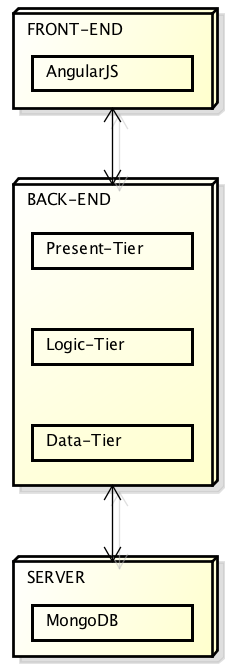
\includegraphics[height=0.6\textheight]{img/architettura_generale}
	\caption[Architettura generale del sistema]{Architettura generale del sistema}
\end{figure}

\textbf{Presentation-Tier}: contiene il front-end dell'applicazione, che si occupa della presentazione dei dati all'utente. Funge da interfaccia tra l'utente e il back-end, interagendo con il tier sottostante.

\textbf{Logic-Tier}: comunica con il livello superiore elaborando le richieste generate da esso e recuperando i dati dal livello inferiore. Questo strato è a sua volta organizzato con un'architettura three-tier per la gestione del back-end dell'applicazione.

\textbf{Data-tier}: questo livello è costituito dal database dell'applicazione ed è dove vengono memorizzate e recuperate le informazioni. Nel nostro caso il database è di tipo non relazionale.

\newpage

%\printglossaries

\end{document}
